\begin{frame}
    \begin{figure}[H]
        \centering
        \resizebox{\textwidth}{!}{%
            \begin{tikzpicture}[pointnode/.style={circle, fill=black}, node distance=5cm, minimum size=5mm]
                \node[pointnode,
                label=above:{Nadajnik},
                label=below:{$0$}] (N) {};
                \node[pointnode,
                label=above:{Odbiornik 1.},
                label=below:{$-0,5$}] (O1) [left=of N] {};
                \node[pointnode,
                label=above:{Odbiornik 2.},
                label=below:{$0,5$}] (O2) [right=of N] {};
                \draw[-, thin, dotted] (-8,0) -- (8,0);
            \end{tikzpicture}
        }%
    \end{figure}
    \begin{figure}
        \centering
        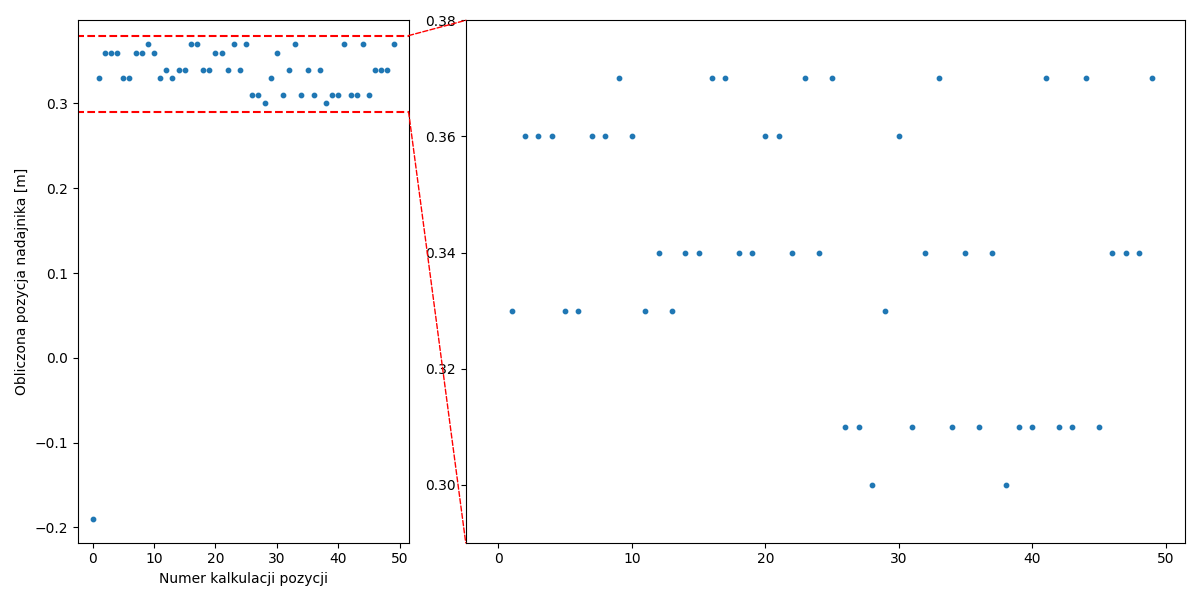
\includegraphics[width=\linewidth]{../pics/mult_lat_1d/position_[0.25]_2.png}
        \caption{Punkt w pozycji (0,25), 2 mikrofony}
    \end{figure}
\end{frame}